\chapter{Backend design} 
\chaptermark{Backend design}

\section{Introduction}
In the previous section, we discussed the prototype for end users. 
In this section, our focus is primarily on the discussion of backend.
This section will focus on how to utilise AI-related tools in the context of the previously mentioned significant prototypes. 
The aim is to facilitate the generation of relevant materials for eBooks production in the administration backend. 
Furthermore, this section will delve into the techniques involved in generating images, audio, and text.

In our last report, we examined the organizational structure of historical  eBooks. 
However, for this particular report, our primary focus shifts towards exploring the application of artificial intelligence (AI) in this domain.

To begin, we have provided a brief overview of our prior research, which primarily centered on the organization of  eBooks. 
It became apparent that different versions and adaptations were necessary to cater to diverse age groups. 
Consequently, we delved into two main approaches aimed at effectively structuring the content.

The first approach involved organizing the material around critical historical events and notable figures, with the objective of offering readers a comprehensive understanding of Māori history. 
This method sought to enrich readers' knowledge of Māori history by delving into the intricacies of historical events and significant personalities.

The second approach focused on aligning the content with local primary and secondary school curricula to ensure its relevance in the education of younger readers. 
Recognizing the importance of addressing the specific needs and developmental stages of these readers, we tailored the content accordingly to resonate with their educational framework.

Building upon our previous research, the forthcoming report will primarily delve into the application of AI techniques within Māori historical  eBooks. 
Specifically, we will explore how AI tools can effectively address the challenges associated with collecting images, audio, and textual resources for these books. 
However, it is imperative to acknowledge the current limitations of AI tools, necessitating caution in their utilisation, particularly in critical areas. 
To ensure the appropriateness of materials, comprehensive guidelines on the effective use of AI tools will be provided. 
Moreover, continuous review and updates of the materials will be conducted to ensure their accuracy and relevance.

\section{How to generate images} 

Currently, generative AI is rapidly advancing, and there are numerous options available for utilising AI-generated images as tools. 
When using AI to generate images, it is important to note that there is no definitive numerical measure to evaluate the similarity between generated images and the training set images in the context of generating adversarial images. 
Objective and subjective criteria are often required to assess the diversity of the images and determine if they are free from obvious inaccuracies. 
Nevertheless, with human intervention, highly acceptable images can be obtained. 

This prototype clearly highlights the issue of a shortage of resources for backgrounds, covers, and illustrations in  eBooks. 
This undoubtedly provides ample opportunities for generative AI to be utilised effectively, significantly reducing the production costs associated with generating eBooks for staff members.

\subsection{Prototype}

In the prototype shown in Fig~\ref{s-1}, a backend administrator has the ability to generate new books using an editor provided in the backend. 
The administrator can extract a portion of text from the editor, which can be in either Māori or English, to serve as the content for generating images. 
Upon clicking a button, the backend system will attempt to generate multiple images in different styles. 
It is then up to the administrator to manually select the best image. 
This design approach helps to mitigate the issue of instability in generative networks' results. 
Furthermore, the manually selected data can be collected and analyzed for statistical purposes. 
In future training iterations, this data can serve as feedback, contributing to a system that better aligns with the desired Māori style.

\begin{figure}[htbp]
  \centerline{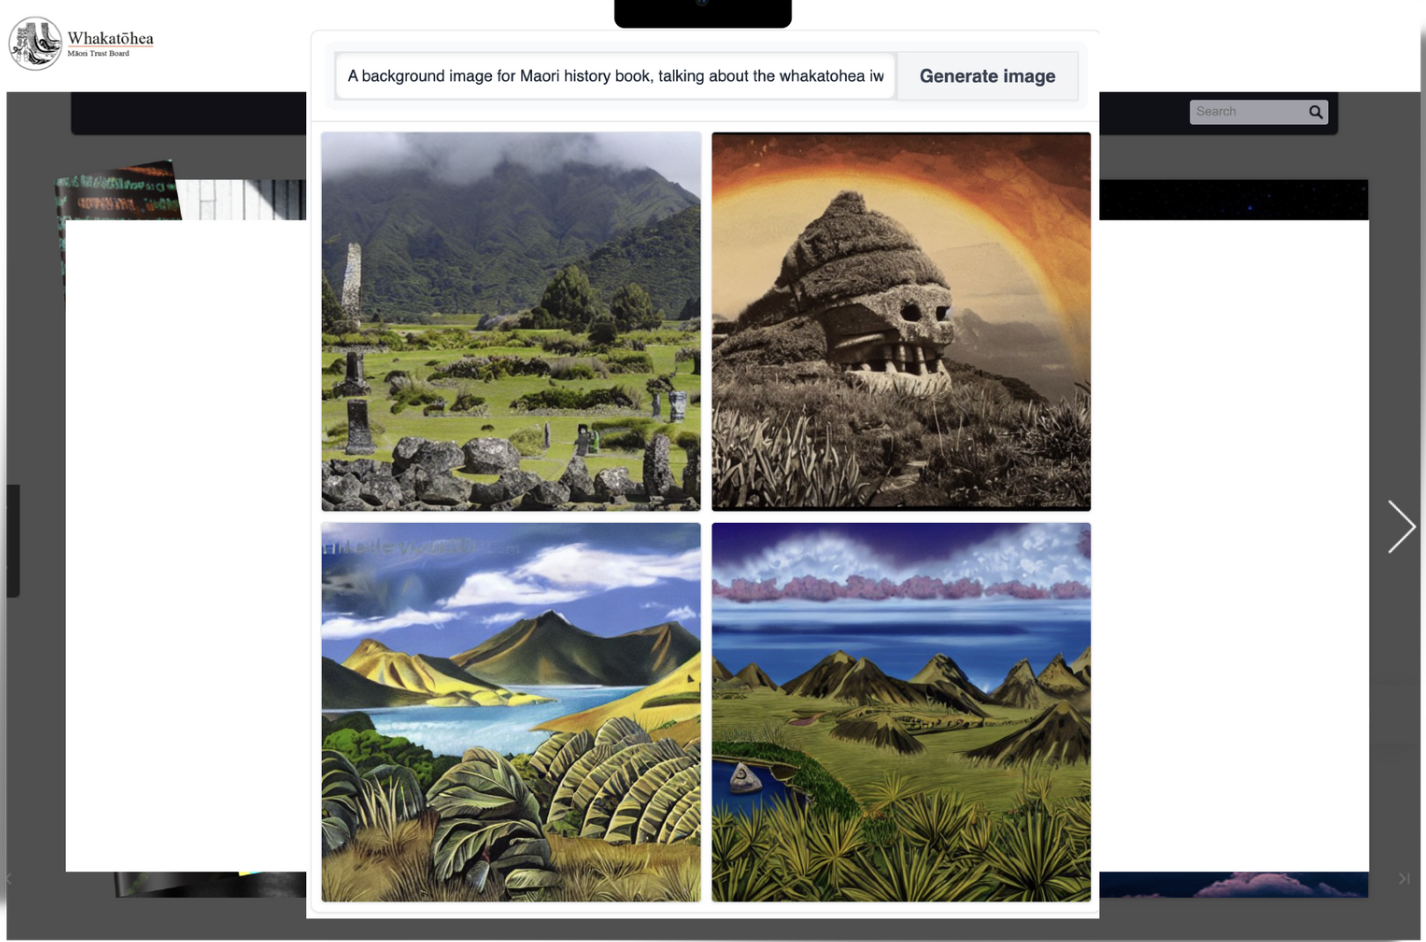
\includegraphics[width=300pt]{images/s-1.png}}
  \caption{Generate images by a backend administrator}
  \label{s-1}
\end{figure}

\subsection{Resources}

Regarding methods for generating meaningful images using generative AI, there are already several excellent commercial services available on the market. 
Among them, DALL·E \autocite{DALL·E99:online} from OpenAI and Stable Diffusion \autocite{StableDi18:online} are particularly well-known. 
Additionally, it is also possible to train such models independently. 
Although this may incur high hardware costs, leveraging cloud computing could potentially be more cost-effective compared to directly using third-party commercial services.
If choosing to manually train such models, it is advisable to consider working based on the open-source project mentioned in this paper \autocite{rombach2021highresolution}.

It is important to note that Māori, being a minority language, may not receive extensive support from many commercial models. 
Additionally, when training models independently, it can be challenging to find sufficient training data for Māori language. 
However, there are some companies that offer models specifically designed for minority languages like Māori. 
For instance, Microsoft claims that their translator provides excellent support for Māori language \autocite{Smartter6:online}.

\section{How to generate audio}

The main scenarios where AI-generated speech is utilised include enabling individuals with visual impairments to navigate through eBooks using voice commands and directly playing the content of the book. 
In this prototype, the envisioned languages include Māori and English. 
This essentially involves the application of text-to-speech and speech-to-text technologies. 
With the continuous advancements in neural networks, these technologies have already achieved remarkable accuracy in addressing English language requirements. 
However, for minority languages, the lack of sufficient accurate resources has posed challenges in finding viable solutions to complete this prototype. 
Fortunately, thanks to the recent release of a new version of a project by Facebook \autocite{Introduc20:online}, which utilised voice data from over 1,100 different languages reading the Bible, highly favorable results have been achieved.

\subsection{Prototype}

The prototype depicted in Fig~\ref{s-2} illustrates a scenario where a visually impaired user is reading an eBook. 
The eBook can be in either Māori or English. 
Through voice commands, the user is able to navigate through the pages and have the book's content played aloud. 
Due to the high accuracy of current models, these operations can be directly performed in the frontend without the need for administrator intervention.

\begin{figure}[htbp]
  \centerline{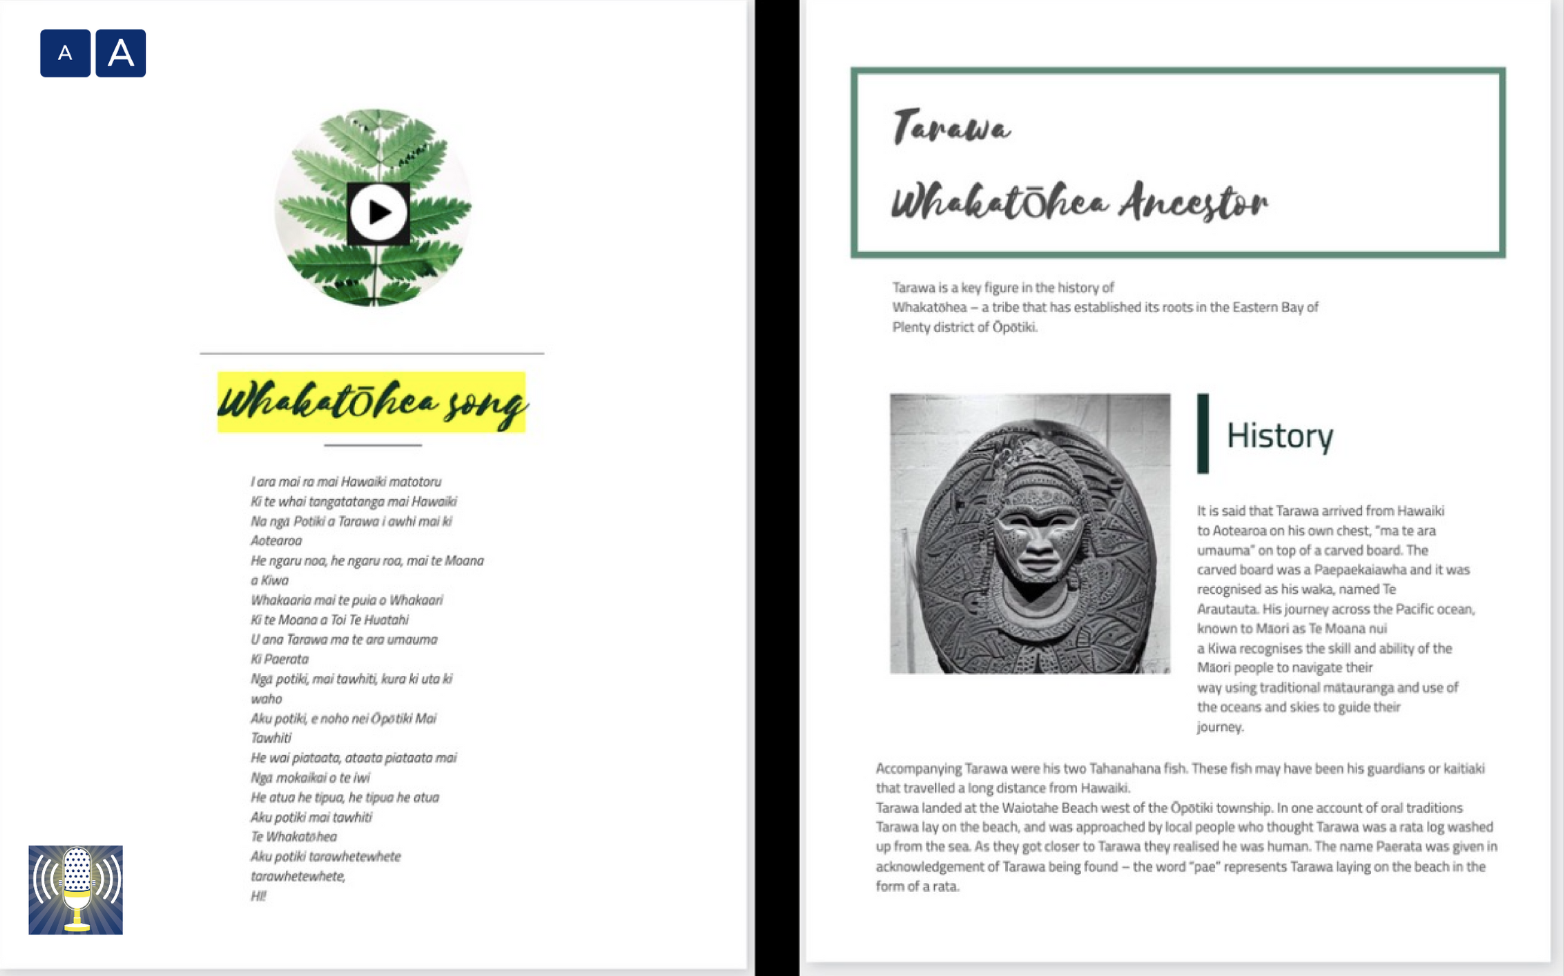
\includegraphics[width=300pt]{images/s-2.png}}
  \caption{Play audio by a enabling individuals}
  \label{s-2}
\end{figure}

\subsection{Resources}

Due to the rapid advancements in AI, timeliness is crucial in selecting appropriate technologies. 
Currently, Facebook's solution appears to be the best option as it can support both Māori and English. 
However, other companies' technologies can also be considered, such as OpenAI's open-source Whisper \autocite{Introduc57:online} or Mozilla's TTS \autocite{mozillaT63:online}. 
It may require collaboration among multiple models to meet the requirements of the prototype, and further research is needed to assess the support for Māori language.

\section{How to generate text}

Today, large language models have gained tremendous popularity. 
Harnessing the power of these models, we can consider utilising their summarization capabilities to generate test questions and answers of varying difficulty levels for our book. 
These can be used as quizzes following the study of the material in the course.

\subsection{Prototype}

The prototype shown in Fig~\ref{s-3} consists of a text excerpt derived from the corresponding book. 
Through this text, the most crucial information can be summarized, and a batch of possible questions and answers can be generated. 

Firstly, the administrator can define the difficulty level, grade level, and the desired number of questions for the current quiz. 
Subsequently, due to the instability of AI model results, it requires backend confirmation by the administrator before saving the questions as test items. 
In this process, the administrator has the ability to modify and delete questions and answers, making the generated quiz more targeted. 
During this process, support for both Māori and English languages should be available, but not all large language models can provide this capability. 
Careful consideration should be given when selecting a model to ensure it meets these requirements.

\begin{figure}[htbp]
  \centerline{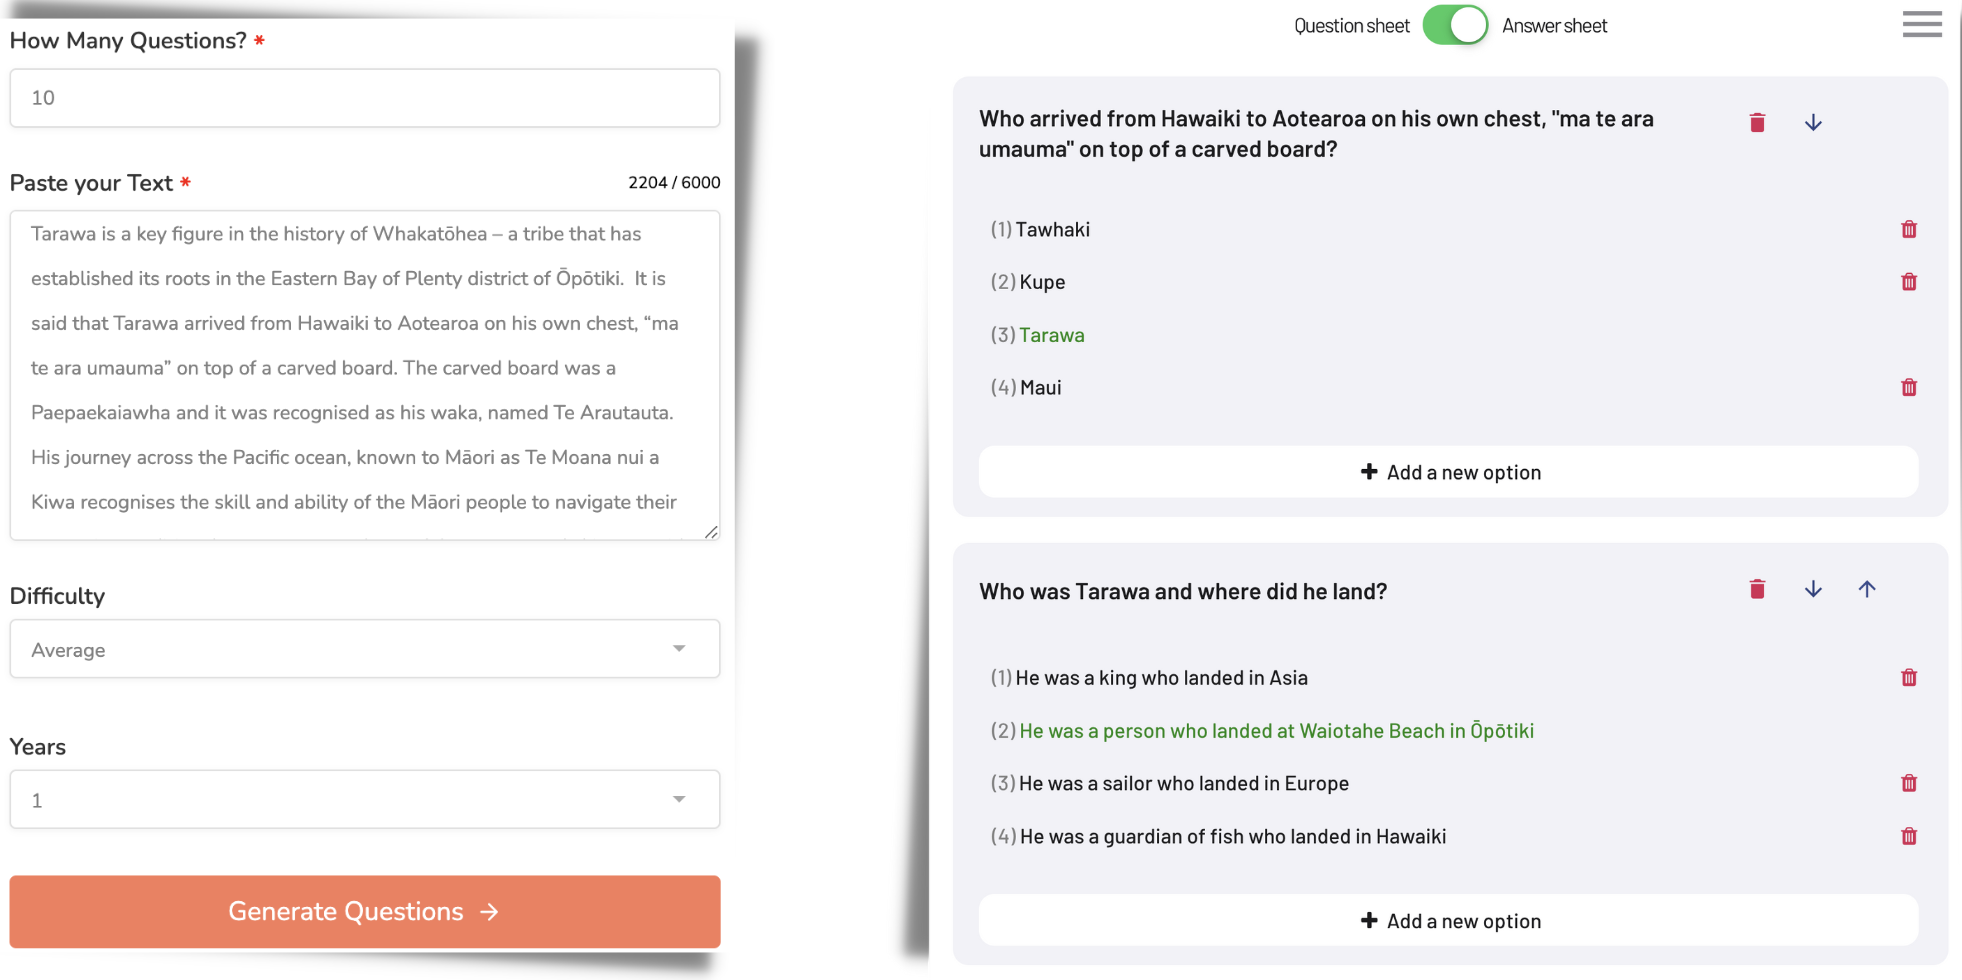
\includegraphics[width=300pt]{images/s-3.png}}
  \caption{Generate quizzes by AI}
  \label{s-3}
\end{figure}

\subsection{Resources}

There are abundant resources available for this task. 
Firstly, one option is to directly utilise the commercial API of ChatGPT, which provides an excellent user experience. 
So far, it is the only system that has achieved comprehensive text summarization and abstraction tasks. 
Secondly, if the chosen solution lacks support for Māori language, Microsoft's Māori language translation mentioned earlier can be integrated. 
This allows for translation into English, followed by question generation. 
Additionally, open-source projects such as Google's T5 model \autocite{roberts2022t5x} can also be considered.

\section{Conclusion}
This section of the report focuses on conducting research on the application of AI in the backend and, in conjunction with the prototype, collecting resources to effectively utilise AI in the frontend and particularly in the backend processes of eBook and test questions generation. 
This simplifies the eBook generation process and provides significant convenience in accurately presenting Māori-related content. 
In the preparation process of eBook materials in collaboration with Whakatōhea iwi, it is believed that this logic will play a crucial role in rapidly establishing the entire framework of Māori history-related content and testing system.

All prototypes mentioned in this section have been implemented and can be accessed through the following URL \autocite{Page1wh37:online}.